\documentclass[18pt]{beamer}
%% SLIDE FORMAT
\usetheme{Boadilla}
\usepackage[utf8]{inputenc}
\usepackage{algpseudocode}
\usepackage{multicol}

\title[Programmieren Tutorium]{9. Programmieren Tutorium:\texorpdfstring{\\}{} Exceptions}
%\subtitle{Fancy Stuff}
\author{Konstantin Zangerle \texorpdfstring{\\}{} info@konstantinzangerle.de}
\date{18. Jan 2016}

\usepackage{listings}
\usepackage{xcolor}

\setlength\columnseprule{.4pt}

\definecolor{mygreen}{rgb}{0,0.6,0}
\definecolor{mygray}{rgb}{0.5,0.5,0.5}
\definecolor{mymauve}{rgb}{0.58,0,0.82}

\lstset{ %
  backgroundcolor=\color{white},   % choose the background color
  basicstyle=\footnotesize,        % size of fonts used for the code
  breaklines=true,                 % automatic line breaking only at whitespace
  captionpos=b,                    % sets the caption-position to bottom
  commentstyle=\color{mygreen},    % comment style
  escapeinside={\%*}{*)},          % if you want to add LaTeX within your code
  keywordstyle=\color{blue},       % keyword style
  stringstyle=\color{mymauve},     % string literal style
  showstringspaces=false,
  language=Java
}
\beamersetuncovermixins{\opaqueness<1>{0}}{\opaqueness<2->{0}} %Dont show things after pause 
% Bibliography

\begin{document}

% change the following line to "ngerman" for German style date and logos
%\selectlanguage{ngerman}

%title page
\begin{frame}
\titlepage
\end{frame}

%table of contents
\begin{frame}{Gliederung}
\tableofcontents
\end{frame}

\section{Organisatorisches}

\begin{frame}{Weihnachten}
 \begin{itemize}
  \item Erstes Tut im neuen Jahr
  \item Noch Tutorien am 25.01., 1.2, 8.2
 \end{itemize}

\end{frame}





\section{Übungsblatt}
\begin{frame}{Übungsschein}
  \large
  Herzlichen Glückwunsch an alle, die jetzt mehr als 60 Punkte haben.
\end{frame}


\section{Command}

\begin{frame}{Command}
 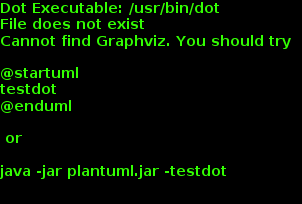
\includegraphics[scale=0.6]{command}
\end{frame}

\begin{section}{Assertions} 
\begin{frame}[fragile]{Assertions}
 \pause
 \begin{itemize}
  \item Müssen über das Compilerflac \verb|-ea| aktiviert werden
  \item Verwenden, wenn irgendwas kaputt ist, falls Assertion nicht erfüllt:
  \begin{itemize}
   \item Nicht als Eingabevalidierung
   \item Gut als Schleifeninvarianten
   \item Vor- Nachbedingung
   \item bei privaten Methoden
  \end{itemize}
 \end{itemize}

\end{frame}
\end{section}


\begin{section}{Unit Tests} 

\begin{frame}{Unit Tests}
\pause
\begin{itemize}
 \item Über JUnit.
 \item Am besten für alle public-Methoden
 \item Möglichkeiten: \begin{itemize}
        \item Überprüfen ob Exception geworfen wird
        \item AssertEquals
        \item AssertTrue /- False
        \item Up and Down Methoden für jeden Testfall und einmalig
       \end{itemize}
\end{itemize}
\end{frame}
\end{section}


\begin{section}{Exceptions} 
\begin{frame}[fragile]{Exceptions}
Ausnahmefälle, die behandelt werden können.
Wichtige Regeln:
\begin{itemize}
 \item Kein \verb|catch Exception e|
 \item Niemals auf Throwable oder Error catchen!
 \item Eigene Exceptions erben von Exception
 \item Throws Deklaration zusammen mit Javadoc verwenden
\end{itemize}

\end{frame}
\end{section}



\begin{section}{Generics} 
\begin{frame}[fragile]{Generics}
 Um Schreibarbeit zu ersparen.
 Oder ist ArrayListInt, ArrayListDouble, ArrayListString, usw schöner als \verb|ArrayList<T>| ?
\end{frame}
\end{section}



\begin{section}{Was noch} 
\begin{frame}{Was noch?}
\begin{itemize}
 \item Debugging mit Eclipse
 \item Sortierverfahren
\end{itemize}
 
\end{frame}
\end{section}



\begin{frame}{Frohe Weihnachten}
 
 Quelle: http://xkcd.com/835
\end{frame}
\end{document}
